\RequirePackage{lineno}
\documentclass[aps,prc,preprint,superscriptaddress,showpacs,showkeys]{revtex4-1}
\usepackage{graphicx}

\begin{document}

\linenumbers

\title{{\Large $J/\psi$ production in PbPb collisions at $\sqrt s_{NN}$ =  2.76 TeV }}

\author{\large V. Kumar}
\author{\large P. Shukla}
\email{pshukla@barc.gov.in}
\affiliation{Nuclear Physics Division, Bhabha Atomic Research Center, Mumbai, India}
\affiliation{Homi Bhabha National Institute, Anushakti Nagar, Mumbai, India}

\date{\today}


\begin{abstract}

 In this work we calculate the $J/\psi$ suppression and regeneration in quark gluon plasma.
The $J/\psi$ suppression is estimated using gluon dissociation in medium. The rate of 
regeneration has been calculated using detailed balance. 
 
 
 

\end{abstract}

\pacs{12.38.Mh, 24.85.+p, 25.75.-q}

\keywords{quark-gluon plasma, kinetic equation}


\maketitle


\section{Introduction}

%%%% Taken from Upsilon ratio paper  %%%%%%%%%%%

   The heavy ion collisions produce matter at extreme temperatures and densities where 
it is expected to be in the form of Quark Gluon Plasma 
(QGP), a phase in which the quarks and gluons can move far beyond  the size of a nucleon 
making color degrees of freedom dominant in the medium. 
  The experimental effort to produce such matter started with low energy CERN accelerator 
SPS and evolved through voluminous results 
from heavy ion collision at Relativistic Heavy Ion Collider (RHIC) \cite{INTRO}.
The recent results from Large Hadron Collider (LHC) experiments \cite{QGP_Tc} are 
pointing towards formation of high temperature system in many ways similar to the matter
produced at RHIC. 
  One of the most important signal of QGP is the suppression of 
quarkonium states \cite{SATZ}, both of the charmonium ($J/\psi$, $\psi(2S)$, $\chi_{c}$, etc) 
and the bottomonium ($\Upsilon(1S)$ , $\Upsilon(2S)$, $\chi_{b}$, etc) families. This is thought to be a 
direct effect of deconfinement, when the binding potential between the constituents of a quarkonium state, 
a heavy quark and its antiquark, is screened by the colour charges of the surrounding light quarks and gluons. 
 The ATLAS and CMS experiments have carried out detailed quarkonia measurements in Pb+Pb collisions 
with the higher energy and luminosity available at the LHC.
 The ATLAS measurements \cite{ATLAS} show suppression of inclusive $J/\psi$ with high transverse momenta $p_T$  
in central PbPb collisions compared to peripheral collisions at $\sqrt s_{NN} = 2.76$ TeV. 
  Similarly, CMS measured a steady and smooth decrease of suppression 
of prompt $J/\psi$ as a function of centrality with nuclear modification factor $R_{AA}$ remaining $<$ 1 even 
in the peripheral bin \cite{JCMS}. 
 
 The melting temperature of the quarkonia states depend on their binding energy. The ground states, 
$J/\psi$ and $\Upsilon(1S)$ are expected to dissolve at significantly higher temperatures than the 
more loosely bound excited states. 
   The $\Upsilon(2S)$ and $\Upsilon(3S)$ have smaller binding energies as compared to ground
state $\Upsilon(1S)$ and hence are expected to dissolve at a lower temperature. 
 With the 2011 Pb+Pb run the CMS published results on sequential suppression of 
$\Upsilon(nS)$ states as a function of centrality \cite{CMSU2} with enlarged statistics
over their first measurement \cite{UCMS}, where a suppression of the excited $\Upsilon$ states with respect 
to the ground state have been observed  
in PbPb collisions compared to pp collisions at $\sqrt s_{NN} = 2.76$ TeV.\cite{YSuppAbdShuk}

  The quarkonia yields in heavy ion collisions are also modified due to non-QGP effects such as
shadowing, an effect due to change of the parton distribution functions inside the nucleus,
and dissociation due to nuclear or comover interaction \cite{Vogt}.
  If large number of heavy quarks are produced in initial heavy ion collisions at LHC energy 
this could even lead to enhancement of quarkonia via statistical recombination \cite{Rapp1,Rapp2}. 
   
 In this paper, we calculate the charmonia suppression due to thermal gluon activation  in an expanding
QGP. Another sources which can alter the yield of charmonium are considered e.g. nuclear shadowing 
and gluon saturation. Impact parameter dependence of parton distribution functions is also taken in account
and at last we consider the effect of J/$\psi$ regeneration using the statistical hadronization model.
J/$\psi$ yield is studied as a function of impact parameter or centerality of events. Calculations are compared
with experimental data, where data is available.



\section{Charm production rates}

  
  The large heavy quark mass allows their production to be calculated in 
perturbative QCD.  We calculate the production cross sections for 
$c\overline c$ and  $b\overline b$ pairs to NLO in pQCD  using
the CTEQ6M parton densities \cite{CTEQ6}.  The central EPS09 parameter set 
\cite{EPS09} is used to calculate the modifications of the parton densities in 
Pb+Pb collisions.  
 
 We use the same set of parameters
as that of Ref.~\cite{CNV} with the exclusive NLO calculation of Ref.~\cite{MNR}
to obtain the exclusive $Q \overline Q$ pair rates as well as their decays
to dileptons.  We take $m_c = 1.5$~GeV/$c^2$, $\mu_F/m_T = \mu_R/m_T = 1$ and  
$m_b = 4.75$~GeV/$c^2$, $\mu_F/m_T = \mu_R/m_T = 1$ as the central values for
charm and bottom production respectively.  Here $\mu_F$ is the factorization 
scale, $\mu_R$ is the renormalization scale and $m_T = \sqrt{m^2 + p_T^2}$.  
The mass and scale variations are added in quadrature to obtain the uncertainty
bands \cite{CNV,ContinuumVKShuk}.
    
  
  The production cross sections for heavy flavor at $\sqrt{s_{_{NN}}}= 2.76$ 
TeV are shown in Table~\ref{NLOcros}.  The number of $Q \overline Q$ pairs
in a minimum bias Pb+Pb event is obtained from the per nucleon cross
section, $\sigma_{\rm PbPb}$, by

\begin{eqnarray}
N_{Q \overline Q} = {A^2 \sigma_{\rm PbPb}^{Q \overline Q}  \over  
\sigma_{\rm PbPb}^{\rm tot}} \, \, .
\end{eqnarray}

 At 2.76 TeV, the total Pb+Pb cross section, $\sigma_{\rm PbPb}^{\rm tot}$, 
is 7.65 b \cite{PbPbTotal}.

\begin{table}
\caption[]{Heavy flavor cross sections at 
$\sqrt{s_{_{NN}}}= 2.76$ TeV.  The cross sections are given per nucleon while
$N_{Q \overline Q}$ and $N_{l^+ l^-}$ are the number of $Q \overline Q$ and lepton 
pairs per Pb+Pb event.}
\label{NLOcros}
\begin{tabular}{l|l|l} 
\hline 
                 & $ c \overline c$     &J/$\psi$    \\
                 
\hline
$\sigma_{\rm PbPb}$   & $1.76^{+2.32}_{-1.29}$ mb       & $31.4$ $\mu$b \\
$N_{Q\overline Q}$      & $9.95^{+13.10}_{-7.30}$           & $0.177$     \\

\hline
\end{tabular}
\end{table}


\section{Modification of J/$\psi$ in presence of QGP}

  In Kinetic approach \cite{THEWS} the proper time evolution of the $J/\psi$ population is given by the rate equation 
\begin{equation}\label{eqkin}
{dN_{J/\psi} \over d\tau}  = \lambda_F {N_c N_{\bar c} \over V(\tau)} - \lambda_D N_{J/\psi} \rho_g.
\end{equation}
with $\rho_g$ the number density of gluons, $\tau$ the proper time
and $V(\tau)$ the volume of the deconfined spatial region.
The reactivities $\lambda_{F,D}$ are
the reaction rates $\langle \sigma v_{\mathrm{rel}} \rangle$
averaged over the momentum distribution of the initial
participants, i.e. $c$ and $\bar c$ for $\lambda_F$ and
$J/\psi$ and $g$ for $\lambda_D$.
The gluon density is determined by the equilibrium value in the
QGP at each temperature. 
 The solution of Eq.~(\ref{eqkin}) is given by
\begin{equation}
N_{J/\psi}(\tau_f) = \epsilon(\tau_f) \,N_{J/\psi}(\tau_0)
+\epsilon(\tau_f)\,{N_{c\bar{c}}^2}\int_{\tau_0}^{\tau_f}
{\lambda_{\mathrm{F}} \over V(\tau)\,\epsilon(\tau)} d\tau
\label{eqbeta}
\end{equation}
where $\tau_f$ is the hadronization time determined by the
initial temperature ($T_0$ )  and
final temperature ($T_f$ ).
The function 
\begin{equation}
\epsilon(\tau_f) = e^{-\int_{\tau_0}^{\tau_f}{\lambda_{\mathrm{D}}\,\rho_g\,d\tau}} 
\end{equation}
For a longitudinal isentropic \cite{bj83} expansion the volume is given by

\begin{equation}
V(\tau)=V_o\,{\tau \over \tau_o}
=\pi\,R^{2}\tau_0\,{\tau \over \tau_o}
=\pi\,R^{2}\tau,
\end{equation}
which gives 

\begin{equation}
N_{J/\psi}(\tau_f) = \epsilon(\tau_f)  N_{J/\psi}(\tau_0) 
                  + \epsilon(\tau_f) \,{N_{c\bar{c}}^2 \over \pi R^{2}} \,\int_{\tau_0}^{\tau_f}
{  {\lambda_{\mathrm{F}} \over \tau\,\epsilon(\tau)} d\tau}
\label{eqbeta1}
\end{equation}
 The $R_{AA}$ can be written as 
\begin{equation}
R_{AA} = \epsilon(\tau_f) + \epsilon(\tau_f) \, {N_{c\bar{c}}^2 \over \pi R^{2}\,N_{J/\psi}(\tau_0)} \, \int_{\tau_0}^{\tau_f}
{  {\lambda_{\mathrm{F}} \over \tau\,\epsilon(\tau)} d\tau}.
\label{raa}
\end{equation}
wher $R$ is the spatial extension of quark gluon plasma given by 
\begin{equation}\label{rnpart}
R(N_{\rm part}) = R_0 \, \sqrt{N_{\rm part} \over N_{\rm part0} }.
\end{equation}
The initial temperature as a function of centrality is calculated by 
\begin{equation}\label{InT1}
T(N_{\rm part})^3 = T_0^3 \, \left({dN/d\eta \over N_{\rm part}/2}\right) / \left({dN/d\eta \over N_{\rm part}/2}\right)_{0-5\%},
\end{equation}
where $T_0$ is the initial temperature assumed in 0-5\% centrality and $(dN/d\eta)$
is the multiplicity as a function of number of participants measured by ALICE experiment \cite{MULT}. 
Both ALICE and CMS \cite{CMSmult} measurements on multiplicity agree well with each other.
The initial temperature $T_0$ for 0-5\% central collisions for a given initial time $\tau_0$ is obtained by 

\begin{equation}\label{InT2}
T_{0}^{3}\tau_{0} = \frac{3.6}{4a_{q}\pi R_{0-5\%}^{2}}\left(\frac{dN}{d\eta}\right)_{0-5\%},
\end{equation}
Here $(dN/d\eta)_{0-5\%}$ = 1.5$\times$1600 obtained from the charge particle multiplicity measured in 
Pb+Pb collisions at 2.76 TeV \cite{MULT} and $a_{q}$ = 37$\pi^{2}$/90 is the degrees of freedom we take in 
in quark gluon phase. Using Eq.~(\ref{rnpart}) we can obtain the transverse size of the system
for 0-5\% centrality as $R_{0-5\%}$ = 0.92$R_0$. 
 For $\tau_{0}$ = 0.1 fm/$c$, we obtain $T_{0}$ as 0.62 GeV using Eq.~(\ref{InT2}). 
The critical temperature is taken as $T_{C}$ = 0.160 GeV \cite{QGP_Tc}. 
N$_{J/\psi}(\tau_0)$ and N$_{c\bar{c}}$ in Eq.~(\ref{eqbeta1}) will also be a function of 
centrality. They will scale as number of collision in particular centrality class.
Number of collisions and number of participants can be calculated from Glauber model 
calculations.



%%%%%%%%%%%%%%%%%%%%%%%%%%%%%%%%%%%%%%%%%%%%%%%%%%%%%%%%%%%%%%%%%%%%
\section{Dissociation Rate}
The gluon-$J/\psi$ dissociation cross section is given by \cite{ks95}
\begin{equation}
  \sigma (q^0)= \frac{2\pi}{3}\left(\frac{32}{3}\right)^2
  \left(\frac{16\pi}{3g_s^2}\right)\frac{1}{m^2_Q}
  \frac{(q^0/\epsilon_0-1)^{3/2}}{(q^0/\epsilon_0)^5}\; , \label{eq1}
\end{equation}
where $g_s$ is the coupling constant of gluon and $c$ quark, $m_Q$
the $c$ quark mass, and $q^0$ the gluon energy in the $J/ \psi$ rest
frame;  its value must be larger than the $J/\psi$ binding energy
$\epsilon_0$. Since
for the tightly bound ground state of quarkonium
the binding force between the heavy quark and antiquark
is well approximated by the one-gluon-exchange Coulomb potential,
the $Q\bar{Q}$ bound state is hydrogen-like and the Coulomb relation
holds,
\begin{equation}
\epsilon_0 =\left({3g_s^2 \over 16\pi}\right)^2 m_Q \; . \label{eq2}
\end{equation}
The cross section thus can be rewritten as
\begin{equation}
  \sigma (q^0)=\frac{2\pi}{3}\left(\frac{32}{3}\right)^2
  \frac{1}{m_Q(\epsilon_0 m_Q)^{1/2}}
\frac{(q^0/\epsilon_0-1)^{3/2}}{(q^0/\epsilon_0)^5}\; . \label{eq3}
\end{equation}
As shown in Monte Carlo simulations \cite{KEXW}, the parton
density in the early stage of high-energy heavy-ion collisions
has an approximate Bjorken-type \cite{bj83} scaling behavior. We
will only consider $J/\psi$ suppression in the central rapidity
region ($y_{J/\psi}\simeq 0$). In this case, the $J/ \psi$ will move
in the transverse direction with a four-velocity
\begin{equation}
u=(M_T, \vec{P_T}, 0)/M_{J/\psi}, \label{eq4}
\end{equation}
where $M_T=\sqrt{P_T^2+M^2_{J/ \psi}}$ is defined as the $J/\psi$'s
transverse mass. A gluon with a four-momentum $k=(k^0,\vec{k})$
in the rest frame of the parton gas has an energy $q^0=k\cdot u$
in the rest frame of the $J/\psi$ given by
\begin{eqnarray}
 q^{0} &= &\frac{k^{0}\,m_{T} + \vec{k} \cdot \vec{p_{T}}}{M_{J/\psi}} \nonumber \\
       &= &\frac{s-M_{J/\psi}^{2}}{2\,M_J/\psi}
\end{eqnarray}
The thermal gluon-$J/\psi$ dissociation cross section is then defined as
\begin{eqnarray}
\langle v_{\rm rel} \sigma (k \cdot u)\rangle_k &= &\frac{\int d^3k v_{\rm rel} \sigma (k \cdot u) f(k^0;T)}{\int d^3k f(k^0;T)},
 \label{eq5}
\end{eqnarray}
where the gluon distribution in the rest frame of the parton gas is
\begin{equation}
  f(k^0;T)=\frac{\lambda_g}{e^{k^0/T}-1} \label{eq6}
\end{equation}
The relative velocity $v_{\rm rel}$ between the $J/\psi$ and a gluon is
\begin{eqnarray}
 \langle v_{\rm rel} \sigma (k \cdot u)\rangle_k &= & \frac{P_{J/\psi}\cdot k}{k^0M_T} \\
              &= & 1-\frac{\vec{k}\cdot\vec{P}_T}{k^0M_T} \\
              &= & {s- M_{J/\psi} \over 2E_1E_2}  \\
              \label{eq7}
\end{eqnarray}

Changing the variable to the gluon momentum, $q=(q^0,\vec{q})$, in
the rest frame of the $J/\psi$, the integral in the numerator
of Eq.~(\ref{eq5}) can be rewritten as

\begin{eqnarray}
  \langle v_{\rm rel} \sigma (k \cdot u)\rangle_k   =  \int d^3q \frac{M_{J/\psi}}{M_T}\sigma(q^0) f(k^0;T), 
\label{eq8}
\end{eqnarray}
where

\begin{equation}
  k^0=(q^0M_T+\vec{q}\cdot\vec{P}_T)/M_{J/\psi} \; . \label{eq9}
\end{equation}
putting the value of $k^{0}$ and solving

\begin{eqnarray} 
\langle v_{\rm rel} \sigma (k \cdot u)\rangle_k &= &\frac{M_{J/\psi}}{M_T} \int d^3q \sigma(q^0) \frac{\lambda_{g}} {  e^{ \frac{q^0m_{T}}{M_{J/\psi}T}} e^{ \frac{ \vec{q}\cdot \vec{p_{T} } }{ M_{J/\psi}T }  } -1}  \nonumber \\
&= &\lambda_{g} \frac{M_{J/\psi}}{M_T} \int d^3q \sigma(q^0)   \sum_{n=1}^{\infty}  e^{ \frac{-n\,q^0m_{T}}{M_{J/\psi}T}} e^{  \frac{-n\,\vec{q}\cdot \vec{p_{T}}}{M_{J/\psi}T}}  \nonumber \\
&= &\lambda_{g} \frac{M_{J/\psi}}{M_T}  \sum_{n=1}^{\infty} 2\pi  \int q^2 dq \, \sigma(q^0)\,e^{ \frac{-n\,q^0m_{T}}{M_{J/\psi}T}}  \int_{1}^{-1} e^{  \frac{-n\,q\,p_{T} cos\theta}{M_{J/\psi}T}} d(cos\theta) \nonumber \\
&= &\lambda_{g} \frac{M_{J/\psi}}{M_T} \sum_{n=1}^{\infty} 2\pi  \int q^2 dq \, \sigma(q^0)\,e^{ \frac{-n\,q^0 m_{T}}{M_{J/\psi}T}} 
    [e^{-\frac{nq p_T}{M_{J/\psi}T}} - e^{\frac{nq P_T}{M_{J/\psi}T}}]\,\frac{M_{J/\psi}T}{nq p_T}  \nonumber \\
&= &\lambda_{g} \frac{M_{J/\psi}^2}{M_T} 2\pi \sum_{n=1}^{\infty} \frac{T}{n} \int_{\epsilon_0}^{\infty} q dq \, \sigma(q^0)  \,e^{ \frac{-n\,q^0 m_{T}}{M_{J/\psi}T}} 
    \frac{1}{p_T} \left[e^{\frac{n q p_T}{M_{J/\psi}T}} - e^{- \frac{n q P_T}{M_{J/\psi}T}}\right]\\
\label{dissrate}
\end{eqnarray}
$\sigma(q^0)$ can be written as

\begin{equation}
\sigma(q^{0}) = 4\pi\,\left(\frac{8}{3}\right)^3\,\frac{1}{m_Q^{3/2}}\,\epsilon_0^3 \frac{ (q^0-\epsilon_0)^{3/2}}{(q^0)^5}
\end{equation}
 One can carry out the integral in the denominator,
$\int d^3k f(k^0;T)=8\pi \zeta(3)\lambda_g T^3$, where $\zeta(3) = 1.202$.

The special case of Eq.~({dissrate}) for J/$\psi$ $p_T=0$ is

\begin{eqnarray} 
   \frac{1}{p_T} \left[e^{\frac{n q p_T}{M_{J/\psi}T}} - e^{- \frac{n q P_T}{M_{J/\psi}T}}\right] = {2nq \over M_{J/\psi}T}.
\label{case}
\end{eqnarray}
Using this we get 

\begin{eqnarray} 
 \langle v_{\rm rel} \sigma (k \cdot u)\rangle_k  &= &  \int 4\pi\,q^2\,dq \, \sigma(q^0) \frac{\lambda_{g}} {e^{\frac{q^0}{T}} -1}.
\end{eqnarray}





\begin{figure}
  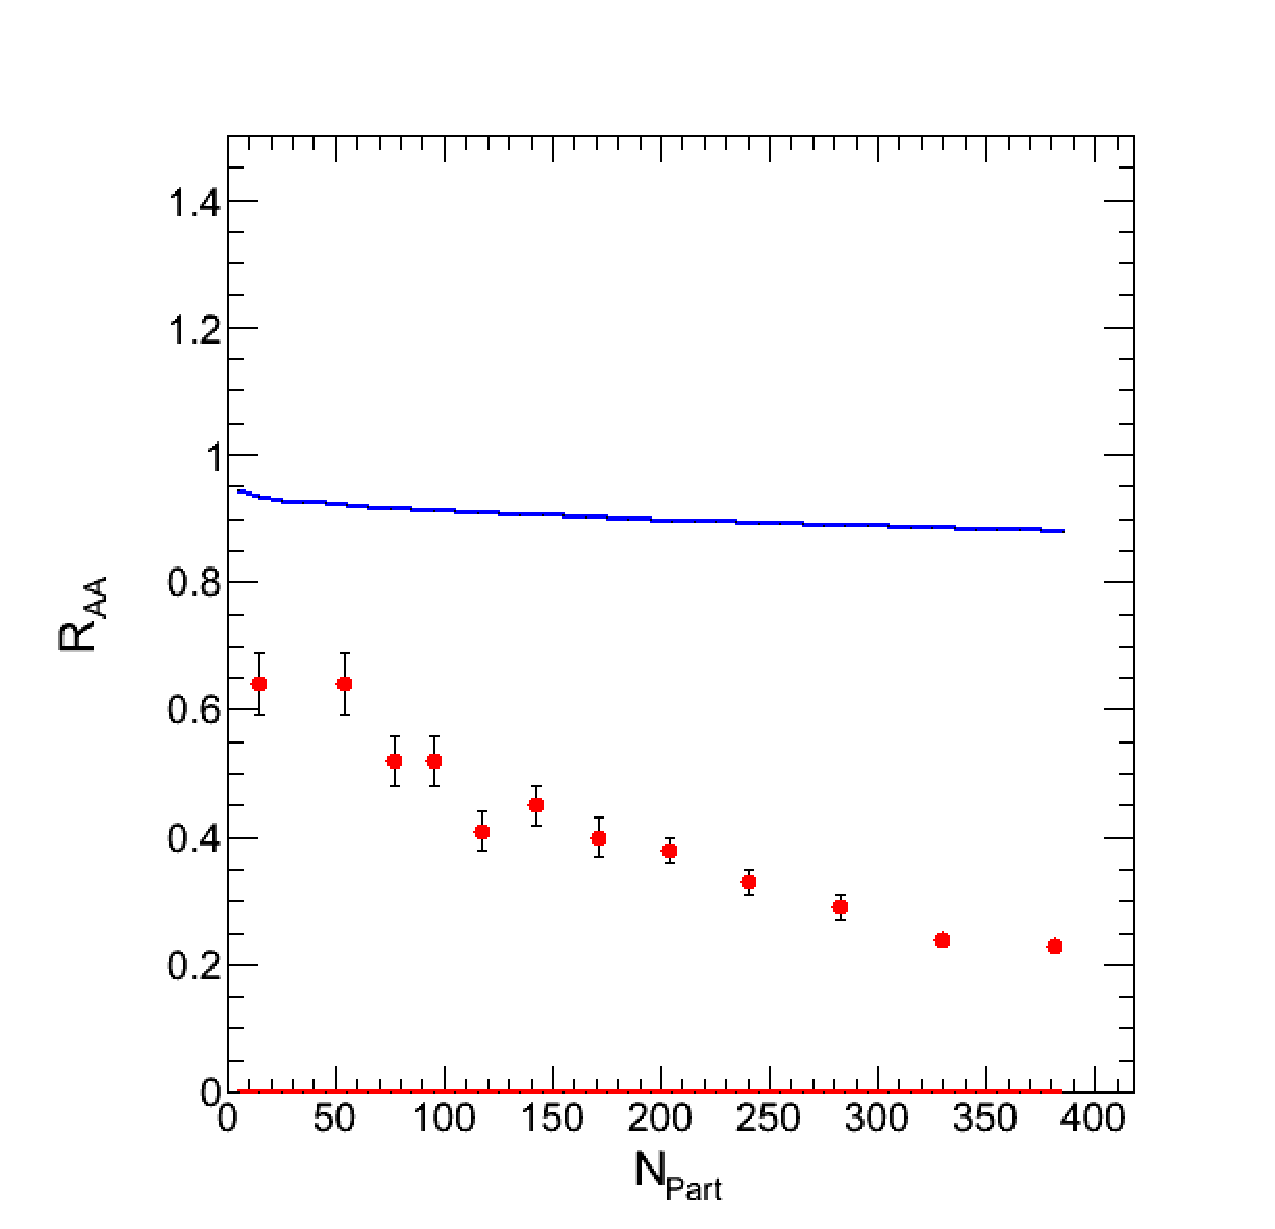
\includegraphics[width=0.48\textwidth]{Raa_21June2_NColl_Tf_Pt65.eps}
  \caption{(Color online)R$_{AA}$ from transport equation compared with CMS data.}
  \label{RaaCMS}
\end{figure}








%%%%%%%%%%%%%%%%%%%%%%%%%%%%%%%%%%%%%%%%%%%%%%%%%%%%%%%%%%%%%%%%%%%%%%%%%%%%%%%%%%%%
\section{Formation Rate}
We can calculate formation rate from dissociation rate using detailed balance relation 
\cite{THEWF} the formation cross section is related to dissociatiob cross section by

\begin{equation}
 \sigma_{F} = \frac{48}{30}\,\sigma_{D}(q^0)\frac{(s-M_{J/\psi})^{2}}{s(s-4m_{c}^{2})}.
\end{equation}
The formation rate can be written as 

\begin{equation}
\lambda_{F} = <\sigma_{F} \,\, v_{\rm rel}>
\end{equation}

v$_{\rm rel}$ is relative velocity between c $\bar{c}$ quark pair and is given by

\begin{eqnarray}
v_{\rm rel} &=& {\sqrt{(p_{1}.p_{2})^{2} - m_Q^{4} } \over E_{1} \, E_{2}} \nonumber \\
            &=& \frac{\sqrt{s(s-4m_{Q}^{2})}}{2E_1E_2}.
\end{eqnarray}
Here
\begin{eqnarray}
 s &= &(E_1+E_2)^{2} - (\vec{p_1}+\vec{p_2})^2 \nonumber \\
   &= & m_Q^{2} + m_Q^{2} + 2 E_1E_2 - 2 |\vec{p_1}||\vec{p_2}|cos\theta 
\end{eqnarray}
where $\vec{p_{1}}$ and $\vec{p_{2}}$ are three momentum of quarks. 

\begin{eqnarray}
\vec{p} = (p sin\theta cos \phi, \, p sin\theta sin \phi, \, p cos\theta)
\end{eqnarray}
The dot product is given by

\begin{eqnarray}
\vec{p_1}.\vec{p_2} &= &|\vec{p_1}||\vec{p_2}|sin \theta_1 sin \theta_2 cos(\phi_1 - \phi_2) + cos \theta_1 cos\theta_2.
\end{eqnarray}
Total expression for formation rate can be written as

\begin{eqnarray}
\lambda_{F} &= &\frac{\int \sigma_{F}(s)\, v_{\rm rel}\,f_{c}(p_1)\, f_{\bar{c}} (p_2) \,d^{3}p_1 \,d^{3}p_2} {\int \,f_{c}(p_1)\,d^{3}p_1 \,\, \int f_{\bar{c}} (p_2)\,d^{3}p_2}\\
            &= &\frac{\int \sigma_{F}(s)\, v_{\rm rel}\,f_{c}(p_1)\, f_{\bar{c}} (p_2) \, 4\pi p_1^{2} dp_1 \, 2\pi p_2^{2} dp_2 d(cos \theta)}
            {4\pi \int p_1^{2} dp_1 \,f_{c}(p_1) \,\, 4 \pi \int p_2^{2} dp_2 \, f_{\bar{c}} (p_2)}.
\end{eqnarray}
Here $\sigma_{F}$ is cross section of c$\bar{c}$ pair going to J/$\psi$ particle.
which is defined as
 \begin{equation}
\sigma_{F} ={ \Theta(q^{2})\,\Theta(4m_{D}^{2}-4m_{c}^{2}-q^{2})\,\sigma(J/\psi) \over N_{c\bar{c}} }
\end{equation}

here $\Theta$(x) is heaviside step function. We take $\sigma_{pp}$ = 7 fm$^{2}$ and
m$_D$ = 1.868 GeV.

and $f_{c}(p)$ and $f_{\bar{c}}(p)$ are parton distribution function of c and $\bar{c}$ respectively.

\begin{equation}
f_{c}(p)={g_c(=6)  \over 1 + {\rm exp} [ { (p^{2} + m^{2} )^{1/2}  \over T }] }.
\end{equation}


\section{Statistical Hadronization Model}

  The heavy quark production at LHC is substantial which may lead to incoherent 
recombination of uncorrelated pairs of heavy quarks and anti quarks which result 
from multiple pair production. In statistical approach \cite{MUNZI} the number of 
J/$\psi$ produced is given by 

  \begin{equation}
N_{J/\psi} = 4 {n_{ch} n_{J/\psi} \over n_{\rm open}^2}  {N_{c\bar c}^2 \over N_{ch} }.
\end{equation}
where $n_i$'s are the thermal densities and $N_{c\bar c}$ is the number of charm pairs produced 
and $N_{ch}$ is the number of total charged 
particle produced. 

The freeze out parameters are $T=170$ MeV and $\mu_B = 0$. For
$dN_{ch}/dy = 1600$ \cite{MULT} and $dN_{c \bar c} /dy = 17.8$, we obtain $dN_{J/\psi} /dy = ?$.
The densities can be calculated using thermal distributions of various particles.

\begin{equation}
n_{open} = {4\pi \,g_{D} \over (2\pi)^{3}} \int_{0}^{\infty} f_{D}(p)p^{2}dp
\end{equation}
by the same method we can calculate the J/$\psi$ number density as

\begin{equation}
n_{J/\psi} = {4\pi \,g_{J/\psi} \over (2\pi)^{3}} \int_{0}^{\infty} f_{J/\psi}(p)p^{2}dp 
\end{equation}
 For total charge particle density we can use 

\begin{equation}
n_{ch} = 2 \,n_{\pi} + 2\, n_{K} + 2\, n_{p},
\end{equation}
where
\begin{equation}
n_{\pi} = {4\pi \,g_{\pi} \over (2\pi)^{3}} \int_{0}^{\infty} f_{\pi}(p)p^{2}dp.
\end{equation}


\section{Cold matter effects}
  The J/$\psi$ can be suppressed due to cold matter effects such as shadowing and due to nuclear
matter and comover interaction.



\section{Summary}



\noindent
\begin{thebibliography}{100}
\medskip
\bibitem{INTRO} I. Arsene {\it et al.} [BRAHMS Collaboration], Nucl. Phys. A {\bf 757}, 1 (2005); 
  B.B. Back {\it et al.} [PHOBOS Collaboration], Nucl. Phys. A {\bf 757} 28.(2005); 
  J. Adams {\it et al.} [STAR Collaboration], Nucl. Phys. A {\bf 757}, 10.(2005); 
  K. Adcox {\it et al.} [PHENIX Collaboration], Nucl. Phys. A {\bf 757} 184 (2005).
\bibitem{QGP_Tc} B. Muller, J. Schukraft and B. Wyslouch, Ann. Rev. Nucl. Part. Sci., arXiv:1202.3233 [hep-ex].
\bibitem{SATZ} T. Matsui and H. Satz, Phys. Lett. B{\bf 178}, 416 (1986).
\bibitem{ATLAS} G. Aad {\it et al.} [ATLAS Collaboration], Phys. Lett. B{\bf 697},294 (2011); arXiv:1012.5419.
\bibitem{JCMS} S. Chatrchyan {\it et al.} [CMS Collaboration]
 J. High Energy Phys. {\bf 1205}, 63 (2012);  arXiv: 1201.5069 [nucl-ex]..
\bibitem{CMSU2} CMS Collaboration, CERN-PH-EP-2012-228, arXiv:1208.2826.
\bibitem{UCMS} S. Chatrchyan {\it et al.} [CMS Collaboration] Phys. Rev. Lett. {\bf 107}, 052302 (2011).
\bibitem{YSuppAbdShuk} A. Abdulasalam and P. Shukla, arXiv:1210.7584.

\bibitem{Vogt} R. Vogt, Phys. Rev. C{\bf 81}, 044903 (2010); arXiv:1003.3497.
\bibitem{Rapp1} X. Zhao and R. Rapp, Nucl. Phys. A{\bf 859}, 114 (2011); arXiv:1102.2194. 
\bibitem{Rapp2} X. Zhao and R. Rapp, Phys. Rev. C{\bf 82}, 064905 (2010); arXiv:1008.5328.

\bibitem{CTEQ6} J.~Pumplin, D.~R.~Stump, J.~Huston, H.~L.~Lai, P.~M.~Nadolsky 
and W.~K.~Tung,  JHEP {\bf 0207}, 012 (2002) [arXiv:hep-ph/0201195];
  D.~Stump, J.~Huston, J.~Pumplin, W.~K.~Tung, H.~L.~Lai, S.~Kuhlmann  and J.~F.~Owens,
  JHEP {\bf 0310}, 046 (2003)  [arXiv:hep-ph/0303013].

\bibitem{EPS09} K. J. Eskola, H. Paukkunen and C. A. Salgado, JHEP{\bf 0904}, 065 (2009) [arXiv:0902.4154 [hep-ph]].

\bibitem{CNV} M. Cacciari, P. Nason and R. Vogt, Phys. Rev. Lett.{\bf 95}, 122001 (2005).

\bibitem{MNR} M. L. Mangano, P. Nason, and G. Ridolfi, Nucl. Phys. B{\bf 373}, 295 (1992).

\bibitem{ContinuumVKShuk} V. Kumar, P. Shukla and R. Vogt, Phys. Rev. C{\bf 86}, 054907 (2012).

\bibitem{PbPbTotal} Total PbPb

\bibitem{THEWS} R. L. Thews and J. Rafalski, Nuclear Physics A698, 575 (2002) [arXiv: hep-ph/0104025];
               R. L. Thews, arXiv: hep-ph/0206179.

\bibitem{bj83} J. D. Bjorken, Phys. Rev. D{\bf 27}, 140 (1983). 

\bibitem{MULT} K. Aamodt {\it et al.} [ALICE collaboration], Phys. Rev. Lett. {\bf 106}, 032301 (2011);
          arXiv:1012.1657 [nucl-ex].

\bibitem{CMSmult} S. Chatrchyan {\it et al.} [CMS Collaboration], J. High Energy Phys. {\bf 1108}, 141 (2011);
       arXiv:1107.4800.  

\bibitem{ks95}D.~Kharzeev and H.~Satz, CERN-TH/95-117, BI-TP 95/20,
         {\it Quark-Gluon Plasma II}, R. C. Hwa (Ed.) (World Scientific, Singapore)

\bibitem{KEXW}K.~J.~Eskola and X.-N.~Wang, Phys. Rev. D {\bf 49}, 1284(1994).
 
\bibitem{THEWF} R.L. Thews and M.L. Mangano, arXiv:nucl-th/05050552 (2006).

\bibitem{MUNZI}  Statistical model

\end{thebibliography}

\end{document}
